\documentclass[]{standalone}

\usepackage{../lenses}



\begin{document}
 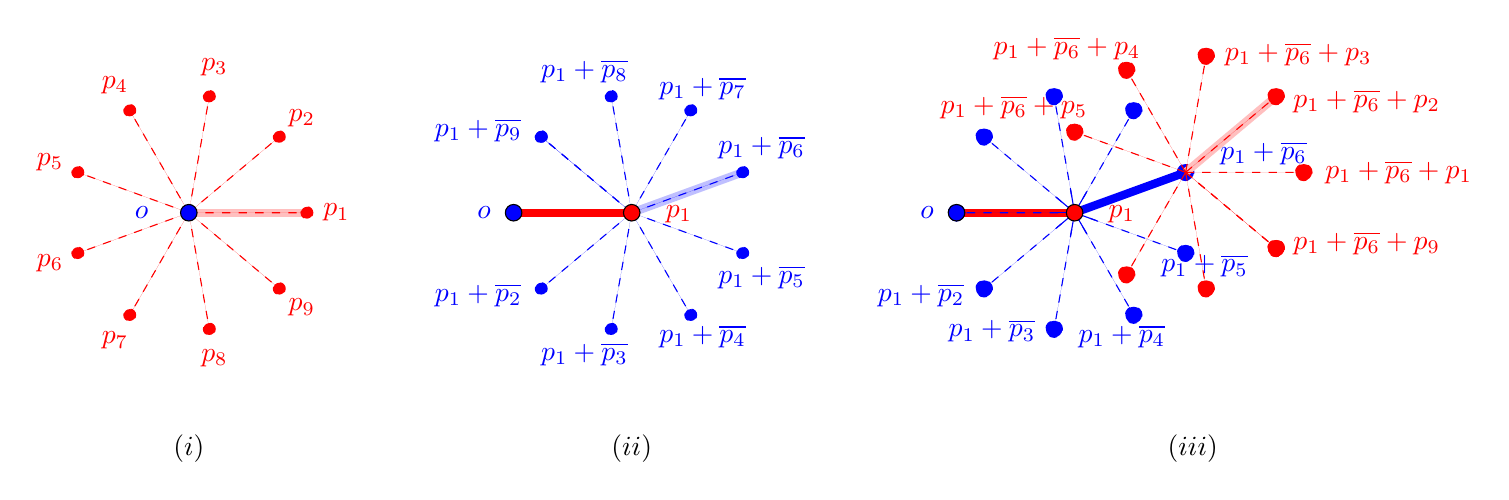
\begin{tikzpicture}
  \begin{scope}[scale=1.5]
  
   \begin{scope}[shift={(0,0)}]
    \draw[line width=3pt,red!25!white](0,0) -- (1,0);
    \foreach \x in {1,2,3,4,5,6,7,8,9} {
     \pgfmathsetmacro{\n}{40*(\x-1)}
     \draw[red,fill=red,dashed](0,0) -- (\n:1) circle(0.05)
      ++(\n:0.25) node{$p_\x$};
    }
    \draw[fill=blue](0,0) circle(0.07) ++(-0.4,+0.0) node[blue]{$o$};

    \path(0,-2) node{$(i)$};
   \end{scope}

   \begin{scope}[shift={(2.75,0)}]
   
    \draw[line width=3pt,red](0,0) -- (1,0);
    \begin{scope}[shift={(1,0)}]
     \draw[line width=3pt,blue!25!white](0,0) -- (20:1);
     \begin{scope}[blue]
      \foreach \x in {0,2,3,4,5,6,7,8,9} {
       \ifthenelse{\x=0}{ } {
        \pgfmathsetmacro{\n}{180+40*(\x-1)}
        \draw[fill=blue,dashed](0,0) -- (\n:1) circle(0.05);
       }
      }
      \draw(+1.1,+0.55) node{$p_1+\overline{p_6}$};
      \draw(+1.1,-0.55) node{$p_1+\overline{p_5}$};
      \draw(+0.6,+1.05) node{$p_1+\overline{p_7}$};
      \draw(+0.6,-1.05) node{$p_1+\overline{p_4}$};
      \draw(-0.4,+1.2) node{$p_1+\overline{p_8}$};
      \draw(-0.4,-1.2) node{$p_1+\overline{p_3}$};
      \draw(-1.3,+0.7) node{$p_1+\overline{p_9}$};
      \draw(-1.3,-0.7) node{$p_1+\overline{p_2}$};
     \end{scope}
    \end{scope}
    \draw[fill=blue](0,0) circle(0.07) ++(-0.25,+0.0) node[blue]{$o$};
    \draw[fill=red](0:1) circle(0.07) ++(+0.4,-0.01) node[red]{$p_1$};

    \path(1,-2) node{$(ii)$};
   \end{scope}

   \begin{scope}[shift={(6.5,0)}]

    \draw[line width=3pt,red](0,0) -- (1,0);

    \begin{scope}[shift={(0:1)}]
     \draw[line width=3pt,blue](0,0) -- (20:1);
     \begin{scope}[blue]
      \foreach \x [count=\c] in {0,2,3,4,5,6,0,0,0} {
       \pgfmathsetmacro{\n}{180+40*(\c-1)}
       \ifthenelse{\x=0}{ 
        \draw(0,0) -- (\n:0.2);
       } {
        \draw[fill=blue,dashed](0,0) -- (\n:1) circle(0.07);
       }
      }
      \draw(+1.6,+0.50) node{$p_1+\overline{p_6}$};
      \draw(+1.1,-0.45) node{$p_1+\overline{p_5}$};
      \draw(+0.4,-1.05) node{$p_1+\overline{p_4}$};
      \draw(-0.7,-1.0) node{$p_1+\overline{p_3}$};
      \draw(-1.3,-0.7) node{$p_1+\overline{p_2}$};

      \begin{scope}[shift={(20:1)}]
       \begin{scope}[red]
        \draw[line width=3pt,red!25!white](0,0) -- (40:1);
        \foreach \x in {1,2,3,4,5,0,7,8,9} {
         \ifthenelse{\x=0}{ } {
          \pgfmathsetmacro{\m}{40*(\x-1)}
          \draw[fill=red,dashed](0,0) -- (\m:1) circle(0.07);
         }
        }
        \draw(+1.10,+0.0) node[right]{$p_1+\overline{p_6}+p_1$};
        \draw(+0.83,+0.6) node[right]{$p_1+\overline{p_6}+p_2$};
        \draw(+0.25,+1.0) node[right]{$p_1+\overline{p_6}+p_3$};
        \draw(-0.30,+1.05) node[left]{$p_1+\overline{p_6}+p_4$};
        \draw(-0.75,+0.55) node[left]{$p_1+\overline{p_6}+p_5$};
        \draw(+0.83,-0.6) node[right]{$p_1+\overline{p_6}+p_9$};
       \end{scope}
      \end{scope}

     \end{scope}
    \end{scope}
    \draw[fill=blue](0,0) circle(0.07) ++(-0.25,+0.0) node[blue]{$o$};
    \draw[fill=red](0:1) circle(0.07) ++(+0.4,-0.01) node[red]{$p_1$};

    \path(2,-2) node{$(iii)$};
   \end{scope}


  \end{scope}
 \end{tikzpicture}
\end{document}